\documentclass{ctexart}
\usepackage{graphicx}

\begin{document}
\title{可行性报告}
\author{马凯,金孜达,刘时,徐亦尧,李文睿}
\setcounter{tocdepth}{2}
\maketitle
\tableofcontents
\newpage

\section{可行性分析}
\subsection{理论依据}
\subsubsection{CAP定理}
CAP定理(CAP theorem),又被称作布鲁尔定理(Brewer's theorem),它指出对于一个分布式计算系统来说,不可能同时满足以下三点:
\begin{itemize}
    \item 一致性(Consistence) (等同于所有节点访问同一份最新的数据副本)
    \item 可用性(Availability)(每次请求都能获取到非错的响应——但是不保证获取的数据为最新数据)
    \item 分区容错性(Network partitioning(英语:Network partitioning)即使任意数量的消息被节点之间的网络丢弃(或延迟),系统仍继续运行(以实际效果而言,分区相当于对通信的时限要求。系统如果不能在时限内达成数据一致性,就意味着发生了分区的情况,必须就当前操作在C和A之间做出选择。)
\end{itemize}

根据定理,分布式系统只能满足三项中的两项而不可能满足全部三项。理解CAP理论的最简单方式是想象两个节点分处分区两侧。允许至少一个节点更新状态会导致数据不一致,即丧失了C性质。如果为了保证数据一致性,将分区一侧的节点设置为不可用,那么又丧失了A性质。除非两个节点可以互相通信,才能既保证C又保证A,这又会导致丧失P性质。

我们的项目抛弃了一致性(C),选择了可用性(A)和分区容错性(P)。

若设备离线,设备获取到的数据存储在本地,如果存储空间已满,系统就会抛弃旧的数据来接收新数据,向系统写入时永远不会报错,但由于旧数据被抛弃,从而失去了一致性。
\subsection{技术依据}
\subsubsection{RIOT OS}
本项目基于 RIOT 实现是可行的。下面给出主要依据。

\paragraph{架构}
RIOT 是微内核架构,整体高度模块化。这为本项目成员理解、修改操作系统代码创造了方便。

\begin{figure}
	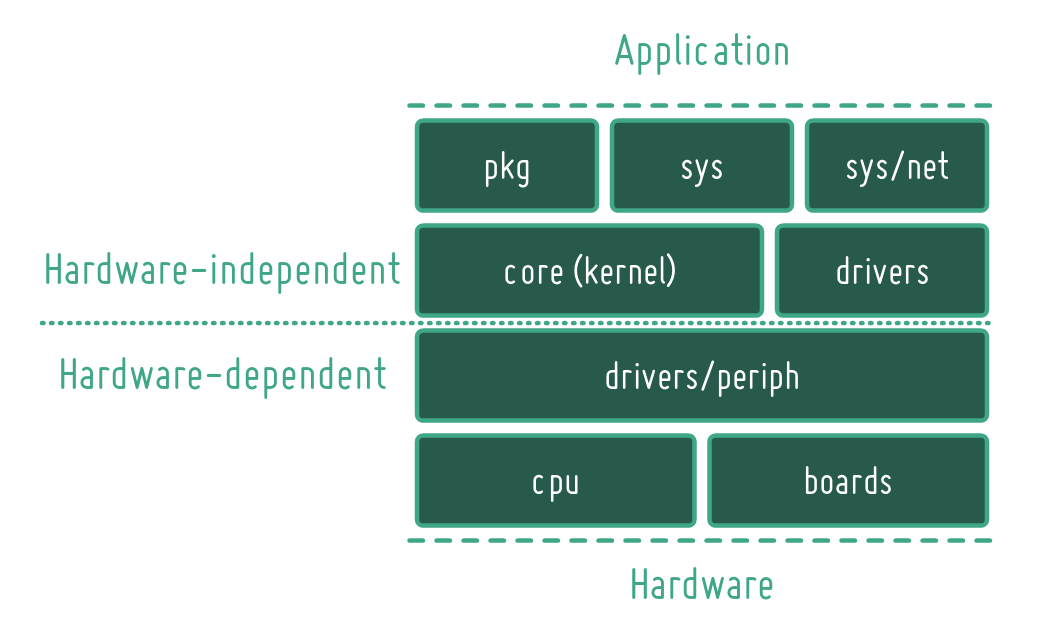
\includegraphics[width=\textwidth]{RIOT-Overview.png}
	\caption{RIOT OS 架构}
	\label{RIOT-Overview}
\end{figure}

\paragraph{资源占用}
RIOT 在极限情况下资源占用极低(见图 \ref{RIOT-Resource}),可以在最苛刻的环境中使用。这对本项目的目标使用场景极为匹配。

\begin{figure}
	\centering
	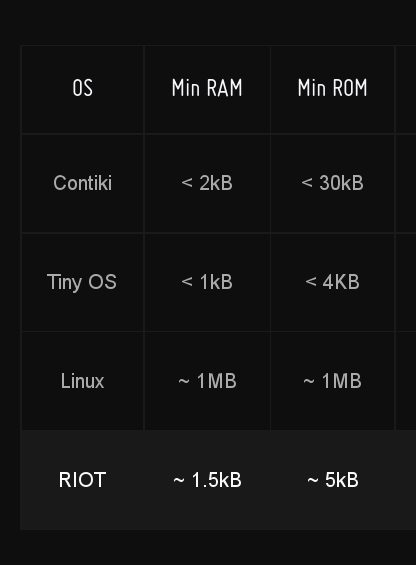
\includegraphics[scale=0.3]{RIOT-Resource.png}
	\caption{RIOT OS 资源占用}
	\label{RIOT-Resource}
\end{figure}


\paragraph{网络栈}
RIOT 提供了完整的网络栈,包括套接字接口和 IP、TCP、UDP 等协议的支持,这为本项目的网络功能实现提供了坚实的基础。RIOT 的模块化设计使得网络协议的替换也更加方便。

\paragraph{调度}
RIOT 调度的基本单位是线程,提供抢占式和协作式两种调度方式,且调度开销很低。基于线程的灵活的调度方式有利于提高可扩展性,也大大方便了成员开展工作。

综上所述,RIOT 为本项目开展提供了极大方便,使得我们无需自己实现这些基础性功能,而是专注于项目本身的创新和设计。

\subsection{创新点}

\section{概要设计报告}

\end{document}